\documentclass[a4paper,12pt]{report}
\usepackage[T2A]{fontenc}
\usepackage[utf8]{inputenc}
\usepackage[english,russian]{babel}
\usepackage{graphicx}
\usepackage{wrapfig}
\usepackage{mathtext} 				% русские буквы в фомулах
\usepackage{amsmath,amsfonts,amssymb,amsthm,mathtools} % AMS
\usepackage{icomma} % "Умная" запятая: $0,2$ --- число, $0, 2$ --- перечисление
\usepackage{capt-of}
\usepackage{appendix}
\usepackage{multirow}
\usepackage{hyperref}
\usepackage{floatrow}
\usepackage[left=2cm,right=2cm,
    top=2cm,bottom=2cm,bindingoffset=0cm]{geometry}
\usepackage{multicol} % Несколько колонок
\usepackage{gensymb}
\title{Отчёт по лабораторной работе №4.3.1. 

Изучение дифракции света.}
\author{Плюскова Н.А. Б04-004 }
\date{\today}
\begin{document}
\maketitle
\section*{1. Аннотация}
В работе исследуется дифракция Френеля и Фраунгофера (на одной и двух щелях), а также изучается влияние дифракции на разрешающую способность оптических инструментов. 

\section*{2. Теоретические сведения и экспериментальные установки}
\subsection*{А. Дифракция Френеля}
\begin{figure}[h]
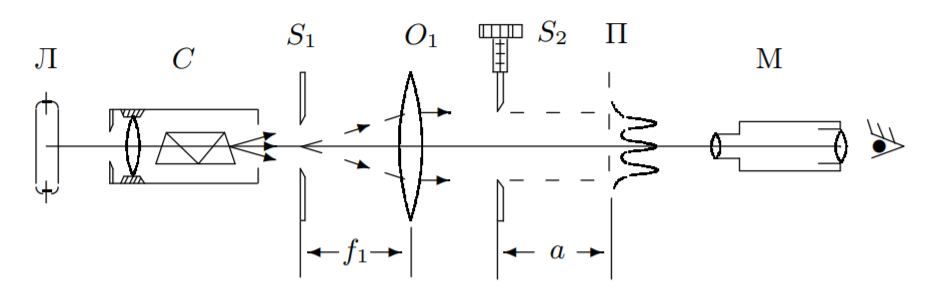
\includegraphics[scale=0.7]{0.png}
\centering
\caption{Схема установки 1.}
\end{figure}
Схема установки представлена на Рис. 1. Световые лучи освещают щель $S_2$ и испытывают на ней дифракцию. Дифракционная картина рассматривается с помощью микроскопа М, сфокусированного на некоторую плоскость наблюдения П. Щель $S_2$ освещается параллельным пучком монохроматического света с помощью коллиматора, образованного объективом $O_1$ и щелью $S_1$, находящейся в его фокусе. На $S_1$ сфокусированно изображение спектральной линии, выделенной из спектра ртутной лампы Л при помощи монохроматор $C$, в котором используется призма прямого зрения. \\
Распределение интенсивности света в плоскости П рассчитаем с помощью зон Френеля. При освещении $S_2$ параллельным пучком лучей (плоская зона) зоны Френеля представляют собой плоскости, параллельные краям щели. Результирующая амплитуда в точке наблюдения определеяется суперпозицией колебаний от тех зон Френеля, которые не перекрыты створками щели. Графическое определение результирующей амплитуды производится с помощью векторной диаграммы -- спирали Корню. Суммарная ширина $m$ зон Френеля $z_m$ определяется соотношение
\begin{equation}
z_m = \sqrt{am\lambda},
\end{equation}
где $a$ -- расстояние от щели до плоскости П. Вид наблюдаемой картины определяется \textit{числом Френеля} $\Phi$:
$$
\Phi^2 = \dfrac{D}{\sqrt{a\lambda}}
$$
-- число зон Френеля, которые укладываются в ширине щели $D$. $p = \frac{1}{\Phi^2}$ называется \textit{волновым параметром}. Дифракционной картины нет, когда П совпадает с плоскостью щели. При малом удалении от щели $\Phi \gg 1$ и картина наблюдается в узкой убласти на границе света и тени у краёв экрана. При последующих удалениях две группы дифракционных полос перемещаются независимо и каждая образует картину дифракции Френеля на экране. Распределение интенсивности может быть найдено с помощью спирали Корню. При дальнейшем увеличении $a$ две системы полос сближаются и накладываются друг на друга, распределение интенсивности определяется числом зон Френеля в полуширине щели. Если их $m$, то будет набюдаться $m-1$ тёмная полоса.
\subsection*{Б. Дифракция Фраунгофера на щели}
\begin{wrapfigure}{r}{0.5\textwidth}
  \begin{center}
    \includegraphics[width = 1\textwidth]{2.png}
  \end{center}
  \caption{Построение зон Френеля}
  \vspace{+5pt}
\end{wrapfigure}
Для выкладок ниже нам потребуется знать \textit{принцип Гюйгенса-Френеля}. Он формулируется следующим образом:\\
\textit{Каждый элемент волнового фронта можно рассматривать как центр  вторичного возмущения, порождающего вторичные сферические волны, а результирующее световое поле  в каждой точке пространства будет определяться интерференцией этих волн.}\\
Теперь рассмотрим первое применение этого принципа, получившее название \textit{метод зон Френеля}

\begin{wrapfigure}{r}{0.3\textwidth}
  \begin{center}
    \includegraphics[width = 1\textwidth]{1.png}
  \end{center}
  \caption{К фазовым соотношениям при дифракции Фраунгофера}
  \vspace{+13pt}
\end{wrapfigure}

Для этого рассмотрим действие световой волны действующей из точки $A$ в какой-то точке $B$.
В этом случае можно, взяв точку $M_0$ в качестве центра (см. рис. 1), построить ряд концентрических сфер, радиусы которых начинаются с $b$ и увеличиваются каждый раз на половину длины волны $\frac{\lambda}{2}$. При пересечении с плоским фронтом волны $F$ эти сферы дадут концентрические окружности. Таким образом, на фронте волны появятся кольцевые зоны (зоны Френеля) с радиусами $r_1, r_2$ и т. д.

Из геометрических соображений посчитав, можно получить, что 
\begin{equation}
r_i = i \sqrt{a \lambda}
\end{equation}

Картина дифракции упрощается, когда ширина щели становится значительно меньше ширины первой зоны Френеля, т.е. если 
\begin{equation}
D \ll\sqrt{a \lambda} 
\end{equation}	
Это условие всегда выполняется при достаточно большом $a$. В этом случае говорят, что \textit{дифракция Фраунгофера}. Дифракционную картину в этом случае называются \textit{дифракцией Фраунгофера}. При выполнении пункта $(2)$ у нас упрощаются фазовые соотношения, что поясняет рис. 2, в итоге с хорошим приближением можно считать, что разность хода между крайними лучами, приходящими от щели в точке наблюдения $P$, с хорошим приближением равна 
\begin{equation}
\Delta = r_2 - r_1 \approx D \sin \theta \approx D \cdot \theta
\end{equation}
Здесь предполагается, что $\theta$ достаточно мал.
Дифракцию Фраунгофера можно наблюдать на установке Рис. 1, но для удобства к подобной установке добавляется объектив $O_2$.

\begin{figure}[H]
\includegraphics[width = 0.7\textwidth]{3.png}
\centering
\caption{Схема установки 2.}
\end{figure}
Дифракционная картина здесь наблюдается в фокальной плоскости объектива $O_2$. Каждому значению $\theta$ соответствует в этой плоскости точка, отстоящая от оптической оси на расстоянии 
\begin{equation}
X = f_2 \tan \theta \approx f_2 \theta.
\end{equation}
Объектив не вносит разности хода между интерферирующими лучам, поэтому в его фокальной плоскости наблюдается неискажённая дифракционная картина. При $\theta = 0$ разность хода между лучами нулевая, поэтому в центре поля зрения дифракционный максимум. Первый минимум соответствует $\theta_1$ такому, что в точке наблюдения разность хода пробегаем все значения от 0 до $2\pi$. Аналогично рассуждая, для $m$-й полосы
\begin{equation}
\theta_m = \frac{m \lambda}{D}
\end{equation}
Расстояние $X_m$ тёмной полосы от оптической оси из (5) и (6)
\begin{equation}
X_m = f_2m\frac{\lambda}{D}
\end{equation}
\subsection*{В. Дифракция Фраунгофера для двух щелей}
Для наблюдения дифракции Фраунгофера на двух щелях $S_2$ заменим экраном Э с двумя щелями. При этом для оценки влияния ширины входной щели на чёткость вместо $S_1$ поставим щель с микрометрическим винтом.
\begin{figure}[H]
\includegraphics[width = 0.7\textwidth]{4.png}
\centering
\caption{Схема установки 3.}
\end{figure}
Два дифракционных изображения входной щели, одно из которых образовано лучами, прошедшими через левую, а другое -- через правую щели, накладываются друг на друга.
Если входная щель достаточно узка, то дифракционная картина в плоскости П подобна той, что получалась при дифракции на одной щели, однако вся картинка испещерена рядом дополнительных узких полос, наличие которых объясняется суперпозицией световых волн через разные щели. Светлая интерфереционная полоса наблюдается в случаях, когда разность хода равна целому числу длин волн. Таким образом, угловая координата максимума порядка $m$ равна
\begin{equation}
\theta_m = \dfrac{m \lambda}{d},
\end{equation}
где $d$ -- расстояние между щелями. Отсюда расстояние между соседними интерфереционными полосами в плоскости П равно
\begin{equation}
\delta x = f_2 \dfrac{\lambda}{d}
\end{equation}
Число интерференционных полос укладывающихся в области центрального максимума равна отношению ширины главного максимума $\frac{2\lambda f_2}{D}$ к расстоянию между соседними полосами:
\begin{equation}
n = \dfrac{2\lambda f_2}{D} \dfrac{1}{\delta f}= \dfrac{2d}{D}.
\end{equation}
При дифракции света на двух щелях чёткая система интерференционных полос наблюдается только при достаточно узкой ширине входной щели $S$. При увеличении ширины картинка пропадает и появляется вновь, но полосы при этом сильно размыты и видны плохо.
\subsection*{Г. Влияние дифракции на разрешающую способность оптического инструмента}
\begin{figure}[H]
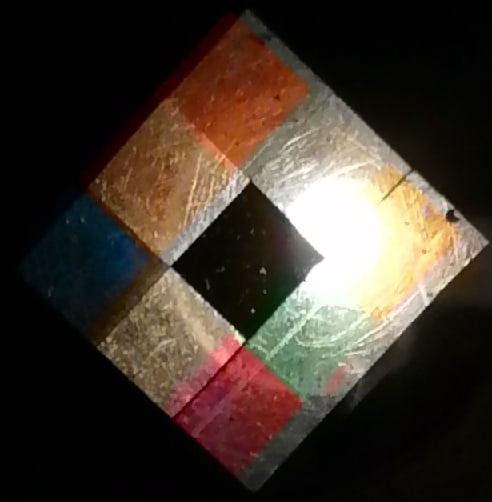
\includegraphics[width = 0.8\textwidth]{5.png}
\centering
\caption{Схема установки 4.}
\end{figure}
В отсутствие щели $S_2$ линзы $O_1$ и $O_2$ создают на плоскости П изоюражение щели $S_1$ и это изображение рассматриваются микроскопом М. Таким образом, установку можно рассматривать как оптический инструмент, предназначенные для получения изображения предмета. Если перед $O_2$ расположить $S_2$, то изображение объекта будет искажено из-за дифракции. Чем меньше ширина щели, тем сильнее искажение. Качественной характеристикой этого искажения может служить $\varphi_{min}$ --- минимальное угловое расстояние между объектами (источниками), которые всё ещё воспринимаются как раздельные. Поместим вместо $S_1$ экран Э с двумя щелями с расстоянием $d$. Тогда на $S_2$ будут падать два пучка света с углом
\begin{equation}
\varphi = \dfrac{d}{f_1}
\end{equation}
Из геометрии расстояние $l$ между изображениями щелей в плоскости П равно 
\begin{equation}
l = \varphi f_2 = d \dfrac{f_2}{f_1}.
\end{equation}
Ширина $\Delta \varphi$ определяется дифракцией на $S_2$. Условия, при которых изображения различимы разные для разных наблюдателей, поэтому используют \textit{критерий Рэлея} -- \textit{максимум одного дифракционного пятна должен совпадать с минимумом другого}. В наших условиях это значит, что угловая полуширина $\frac{\lambda}{D}$ равна угловому расстоянию $\frac{l}{f_2}$.

\section*{3. Ход работы}
Зафиксируем длину волны светофильтра, который используется в схемах вместо монохроматора:
$\lambda = 578$ нм
\subsection*{3.1 Дифракция Френеля }
Определим нуль микрометрического винта щели $S_{2}$, глядя через свет на щель и определив момент ее открытия: $<Z_{0}> = 0,11$ мм.

Добившись наибольшей четкости изображения, зафиксируем начальное положение микроскопа на оптической скамье: $<a_{0}> = 49,25 \pm 0,71$ мм (здесь мы учитывали ширину подставки, на которой стоит микроскоп).
Постепенно отодвигая микроскоп, снимем зависимость а(n), где n - количество наблюдаемый темных полос, m - число зон Френеля, результаты занесем в таблицу 1:

\begin{table}[H]
\begin{tabular}{|c|cccccc|}
\hline
а, см                                   & \multicolumn{1}{c|}{47,75} & \multicolumn{1}{c|}{46,85} & \multicolumn{1}{c|}{46,65} & \multicolumn{1}{c|}{46,45} & \multicolumn{1}{c|}{46,35} & 46,25                      \\ \hline
$\sigma_{a}$, см                             & \multicolumn{6}{c|}{0,71}                                                                                                                                                   \\ \hline
n                                       & \multicolumn{1}{c|}{1}     & \multicolumn{1}{c|}{2}     & \multicolumn{1}{c|}{3}     & \multicolumn{1}{c|}{4}     & \multicolumn{1}{c|}{5}     & 6                          \\ \hline
m                                       & \multicolumn{1}{c|}{2}     & \multicolumn{1}{c|}{3}     & \multicolumn{1}{c|}{4}     & \multicolumn{1}{c|}{5}     & \multicolumn{1}{c|}{6}     & 7                          \\ \hline
2\cdot $z_m$,   мм \cdot 10^{-1}     & \multicolumn{1}{l|}{0,149} & \multicolumn{1}{l|}{0,180} & \multicolumn{1}{l|}{0,208} & \multicolumn{1}{l|}{0,232} & \multicolumn{1}{l|}{0,254} & \multicolumn{1}{l|}{0,274} \\ \hline
$\sigma_{z_{m}}$,   мм \cdot 10^{-1} & \multicolumn{1}{l|}{0,002} & \multicolumn{1}{l|}{0,003} & \multicolumn{1}{l|}{0,003} & \multicolumn{1}{l|}{0,004} & \multicolumn{1}{l|}{0,004} & \multicolumn{1}{l|}{0,004} \\ \hline
\end{tabular}
\caption{Дифракция Френеля}
\end{table}

Измерим ширину щели $S_{2}$, используя окулярную шкалу микроскопа ($D_{2}$), и сравним полученный результат с показанием микрометрического винта щели $S_{2}$ ($D_{1}$): 

\begin{equation}
D_{1} = (257 \pm 1) \text{ мкм}; D_{2} = (270 \pm 10) \text{ мкм}
\end{equation}

Отметим, что результаты сходятся в пределах $2\sigma$

Построим график $2z_{m}(m)$ и отметим на нем ширину щели $S_{2}$:

\begin{figure}[H]
\includegraphics[width = 0.8\textwidth]{2z_m(m).png}
\centering
\caption{График $2\cdot z_{m}(m)$ }
\end{figure}

\subsection*{3.2 Дифракция Фраунгофера на щели }

Добавим в установку собирающую линзу $O_{2}$ с фокусным расстоянием $F_{2} = 9$ см.
Измерим с помощью окулярной шкалы координаты $X_{m}$ нескольких дифракционных минимумов. Полученные результаты занесем в таблицу 2:

\begin{table}[H]
\begin{tabular}{|c|ccccc|}
\hline
$X_{m}$,мкм        & \multicolumn{1}{c|}{5130} & \multicolumn{1}{c|}{5020} & \multicolumn{1}{c|}{4300} & \multicolumn{1}{c|}{4130} & 3580 \\ \hline
$\sigma_{X_{m}}$, мкм & \multicolumn{5}{c|}{10}                                                                                              \\ \hline
m             & \multicolumn{1}{c|}{+2}   & \multicolumn{1}{c|}{+1}   & \multicolumn{1}{c|}{0}    & \multicolumn{1}{c|}{-1}   & -2   \\ \hline
\end{tabular}
\caption{Дифракция Фраунгофера на щели}
\end{table}

Определим ширину щели $S_{2}$ с помощью микрометрического винта ($D_{1}$) и окулярной шкалы ($D_{2}$): 

\begin{equation}
D_{1} = (276 \pm 1) \text{ мкм}; D_{2} = (298 \pm 10) \text{ мкм}
\end{equation}

Построим график зависимости $X_{m}(m)$, по углу наклона прямой которого мы определим ширину щели $D_{3}$:

\begin{figure}[H]
\includegraphics[width = 0.8\textwidth]{X_m(m).jpg}
\centering
\caption{График $X_{m}(m)$ }
\end{figure}


\begin{equation}
X_{m} = m\frac{\lambda}{D_{3}}f_{2}
\end{equation}

Отсюда получаем, что $D_{3} = (261 \pm 16)$ мкм где

\begin{equation}
\sigma_{D_{3}} = \lambda f_{2}\cdot\frac{\sigma_{k}}{k^2},
\end{equation}
 где k - угол наклона касательной
 
 Отметим, что значения ширины щели, полученные разными способами, совпадают в пределах $2\sigma$
 
\subsection*{3.3 Дифракция Фраунгофера на двух щелях }
 
Заменим щель $S_{1}$ щелью $S_{2}$ и добавим экран Э с двумя щелями между линзами $O_{1}$ и $O_{2}$, с фокусными расстояниями $F_{1} = 12,5$ см и $F_{2} = 9$ см соответственно.

Определим с помощью окулярной шкалы микроскопа ширину центрального максимума $\Delta X$ и посчитаем количество светлых промежутков N между самыми удаленными темными полосами внутри центрального максимума: $\Delta X = 0,82 \pm 0,01$ мм, $N = 7\pm 1$

Из формулы 9 найдем расстояние между щелями $d_{1}$: $d_{1} = 0,83 \pm 0,03$ мм. Это значение сходится в пределах $\sigma$ с измеренным нами $d_{2} = (0,79 \pm 0,01)$ мм

Рассчитаем ширину одной щели D по формуле:

\begin{equation}
D = 2f_{2}\cdot\frac{\lambda}{d} = (174 \pm 16)\text{мкм}
\end{equation}

Отсюда получим число полос внутри по формуле 10 : 

\begin{equation}
N = \frac{2d}{D} = 9,3 \pm 0,8 = 9 \pm 1
\end{equation}

Полученное значение сходится с измеренным $N = 7\pm 1$ в пределах $\sigma$.

Измерим ширину входной щели $b_{0} = (144 \pm 10)$ мм, при которой происходит первое исчезновение интерференционных полос, и сравним с результатами расчетов по формуле:

\begin{equation}
\frac{b_{0}}{f_{1}} = \frac{\lambda}{d}, \text{ откуда } b_{0} = (91 \pm 2) \text{ мкм}
\end{equation}

Заметим, что полученные данные сходятся в пределах $5\sigma$

\subsection*{3.4 Влияние дифракции на разрешающую способность оптического инструмента}

Поставим между линзами щель $S_{2}$ и, уменьшая ее ширину, пронаблюдаем за ухудшением качества изображения. Подберем ширину  щели $S_{2}$ так, чтобы изображения обеих щелей почти сливались, но все-таки еще воспринимались отдельно. Запишем показания микрометрического винта щели $S_{2}$: $D_{0} = (0,209 \pm 0,01)$ мм.

Поставим двойную щель перед микроскопом и измерим с помощью окулярной шкалы расстояние d между щелями и ширину каждой щели:

\begin{equation}
d = (0,79 \pm 0,01) \text{ мм }, D_{1} = (0,21\pm 0,01)\text{ мм }, D_{2} = (0,29\pm 0,01)\text{ мм }
\end{equation}

\section*{4. Выводы}

В ходе работы было изучено явление дифракции света - дифракция Френеля на щели, дифракция Фраунгофера на одной и двух щелях, а также исследовано влияние дифракции на разрешающую способность оптического инструмента.

При исследовании явления дифракции Френеля на щели убедились, что ширина зон Френеля примерно равна ширине щели
    
При исследовании явления дифракции Фраунгофера на щели получили значение ширины щели, примерно равно измеренному непосредственно с помощью окулярной шкалы микроскопа:
\begin{center}
 $D_{1} = (276\pm 1) $мкм \hspace{1cm} $D_{2} = (298\pm 10)$ мкм
\end{center}
    
При исследовании явления дифракции Фраунгофера на двух щелях было получено значение расстояния между щелями, примерно равное измеренному с помощью той же окулярной шкалы микроскопа:
    
\begin{center}
$d_1 = (0,83\pm 0,01)$ мм \hspace{1cm} $d_2 = (0,79 \pm 0,01)$ мм
\end{center}

При исследовании влияния дифракции на разрешающую способность оптического инструмента была получена ширина двух щелей:

\begin{center}
$D_1 = (0,21\pm 0,01)$ мм \hspace{1cm} $D_2 = (0,29 \pm 0,01)$ мм
\end{center}
	
\end{document}
